\documentclass[12pt]{article}
 
\usepackage[margin=1in]{geometry}
\usepackage{amsmath,amsthm,amssymb, mathtools}
\usepackage[T1]{fontenc}
\usepackage{lmodern}
\usepackage{fixltx2e}
\usepackage[shortlabels]{enumitem}
\usepackage{mathrsfs}
\usepackage{kbordermatrix}


\usepackage{graphicx}
\usepackage{bbm}

\DeclarePairedDelimiter{\ceil}{\lceil}{\rceil}

\renewcommand{\kbldelim}{(}% Left delimiter
\renewcommand{\kbrdelim}{)}% Right delimiter
 
\newcommand{\N}{\mathbb{N}}
\newcommand{\R}{\mathbb{R}}
\newcommand{\Z}{\mathbb{Z}}
\newcommand{\Q}{\mathbb{Q}}
 
\newenvironment{theorem}[2][Theorem]{\begin{trivlist}
\item[\hskip \labelsep {\bfseries #1}\hskip \labelsep {\bfseries #2.}]}{\end{trivlist}}
\newenvironment{lemma}[2][Lemma]{\begin{trivlist}
\item[\hskip \labelsep {\bfseries #1}\hskip \labelsep {\bfseries #2.}]}{\end{trivlist}}
\newenvironment{exercise}[2][Exercise]{\begin{trivlist}
\item[\hskip \labelsep {\bfseries #1}\hskip \labelsep {\bfseries #2.}]}{\end{trivlist}}
\newenvironment{problem}[2][Problem]{\begin{trivlist}
\item[\hskip \labelsep {\bfseries #1}\hskip \labelsep {\bfseries #2.}]}{\end{trivlist}}
\newenvironment{question}[2][Question]{\begin{trivlist}
\item[\hskip \labelsep {\bfseries #1}\hskip \labelsep {\bfseries #2.}]}{\end{trivlist}}
\newenvironment{corollary}[2][Corollary]{\begin{trivlist}
\item[\hskip \labelsep {\bfseries #1}\hskip \labelsep {\bfseries #2.}]}{\end{trivlist}}
\newcommand{\textfrac}[2]{\dfrac{\text{#1}}{\text{#2}}}
\newcommand{\floor}[1]{\left\lfloor #1 \right\rfloor}

\newenvironment{amatrix}[1]{%
  \left(\begin{array}{@{}*{#1}{c}|c@{}}
}{%
  \end{array}\right)
}

\DeclareMathOperator*{\E}{\mathbb{E}}


\begin{document}

\title{Stochastic Processes II: Midterm}

\author{Chris Hayduk}
\date{March 25, 2021}

\maketitle

\begin{problem}{I}
\end{problem}

\begin{problem}{II}
\end{problem}

Consider a random walk on the square $\{0, 1\}^2$ as a starting point. Then, with initial state $\vec{0} = (0, 0)$, we have the following drawing:

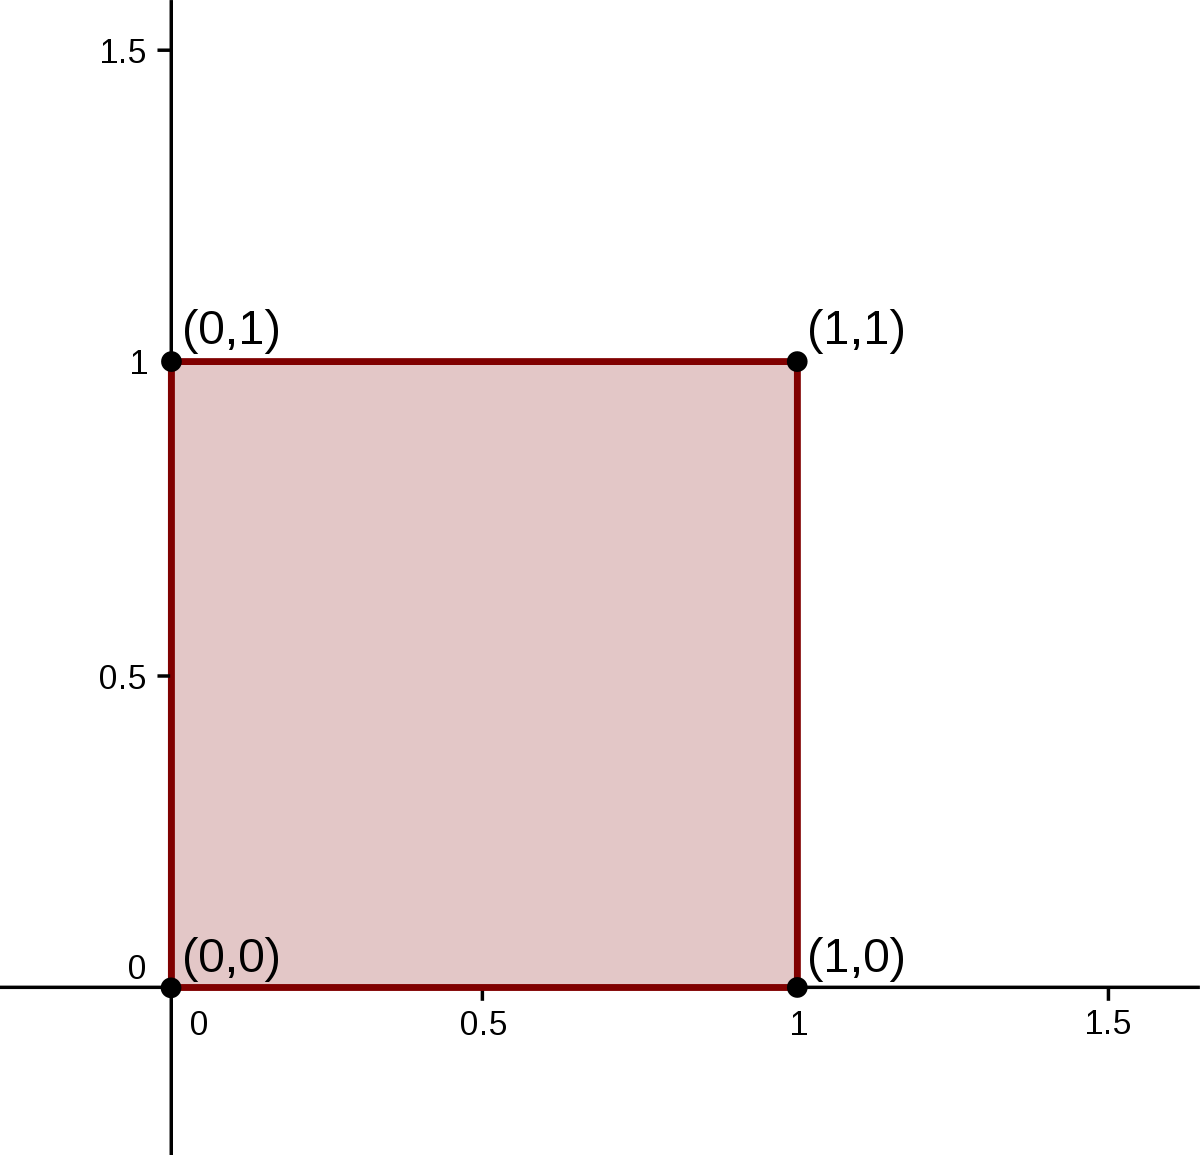
\includegraphics[scale=0.15]{unit_square}

Clearly we have that $(1, 1)$ is the farthest point from our start state, $(0, 0)$. Hence, we would expect to visit $(1, 1)$ the least and this find that $p^t(\vec{0}, \vec{1})$ is minimal for large $t$ in the case of the square. Now consider the cube in $\{0, 1\}^3$:

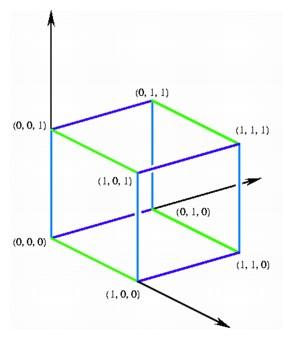
\includegraphics[scale=1]{unit_cube}

Again, we see that it takes the most transitions to reach $(1, 1, 1)$ from the starting point $(0, 0, 0)$. Hence, we would expect to visit $(1, 1, 1)$ the least and this find that $p^t(\vec{0}, \vec{1})$ is minimal for large $t$ in the case of the cube as well.\\

Generalizing this to arbitrary $n$, we would expect that for a lazy random walk on the hypercube $\{0, 1\}$, starting from initial state $\vec{0}$, that $p^t(\vec{0}, \vec{1})$ is minimal for all large $t$. We will prove this now.

\begin{problem}{III}
\end{problem}

\begin{problem}{IV}
\end{problem}

\begin{enumerate}[label=(\Alph*)]

\item Suppose at time $t$, we have reached the point that all cards have been moved. Note that, by definition, the cards in the second deck are moved in the exact same order as the cards in the first deck are. Since every card has been picked by time $t$, every card in the second deck has been picked and moved in accordance with the first deck. Thus, we must have that $X_t = Y_t$ by this time $t$. Thus, we have that,
\begin{align*}
\tau_{\text{couple}} \leq \tau
\end{align*}

\item By Corollary 5.5 and our work above, we have that,
\begin{align*}
t_{\text{mix}} &\leq 4\max_{x,y} \E_{x,y} (\tau_{\text{couple}})\\
&\leq 4\max_{x,y} \E_{x,y} (\tau)
\end{align*}

Note that there is an equal probability of choosing any of the $n$ cards in the deck. That is, each cards is chosen with probability $1/n$. This is precisely the same as the coupon collector problem and so, by Proposition 2.3, we have,
\begin{align*}
E(\tau) = n \sum_{k=1}^n \frac{1}{k}
\end{align*}

Hence, we have that,
\begin{align*}
t_{\text{mix}} \leq 4n \sum_{k=1}^n \frac{1}{k}
\end{align*}

Note that $n \sum_{k=1}^n \frac{1}{k}$ is approximately $n\log(n)$ for large $n$. Hence, for large $n$ we have that,
\begin{align*}
t_{\text{mix}} &\leq \max_{x,y} 4n\log(n)\\
&= 4n\log(n)
\end{align*}
\end{enumerate}

\end{document}